\documentclass[11pt,a4paper]{article}
\usepackage[margin=1.8cm]{geometry}
\usepackage[T1]{fontenc}
\usepackage[utf8]{inputenc}
\usepackage{lmodern}
\usepackage{booktabs,tabularx,array}
\usepackage[colorlinks,urlcolor=blue]{hyperref}
\usepackage{enumitem}
\usepackage{titlesec}
\usepackage{tikz}
\usepackage{pgfplots}
\pgfplotsset{compat=1.18}
\titlespacing*{\section}{0pt}{8pt}{3pt}
\titlespacing*{\subsection}{0pt}{6pt}{2pt}
\setlist{itemsep=1pt,topsep=3pt,leftmargin=1.4em}
\setlength{\parskip}{3pt}
\setlength{\parindent}{0pt}
\newcolumntype{L}{>{\raggedright\arraybackslash}X}
\newcommand{\code}[1]{\texttt{#1}}
\newcommand{\ra}{$\rightarrow$}

\title{RAG Assignment: Baseline Retrieval vs.\ Cross-Encoder Re-Ranking}
\author{Vikash Kumar \quad (Roll No.\ 2025201012)}
\date{19 October 2026}

\linespread{1.3}\selectfont
\begin{document}
\sloppy
\vspace*{-1.4cm}
{\let\newpage\relax\maketitle}
\vspace{-0.9cm}

\textbf{GitHub:} \url{https://github.com/viserion999/LMA_Assignment_1}\\
\textbf{Code:} \code{RAG\_Baseline\_vs\_Reranking.ipynb}\\
\textbf{Outputs:} \code{results/answers.json}, \code{results/llm\_cache.json}

\section*{Setup}
\begin{itemize}
  \item \textbf{Document:} \emph{Magic: The Gathering Comprehensive Rules} (June 2026, 311 pages). I kept only the numbered rules and split them into 971 chunks (one rule + its sub-rules + section heading; median 187 tokens).
  \item \textbf{Models:} Bi-Encoder \code{bge-small-en-v1.5} + FAISS exact cosine search; Cross-Encoder \code{ms-marco-MiniLM-L-6-v2}; LLM \code{gemini-3.5-flash-lite} (temperature 0, same prompt for both pipelines, told to answer only from the context).
  \item \textbf{Queries:} I wrote 49 player-style questions: negation (14), exception (9), keyword trap (10), buried rule (6), control (10). I fixed the gold rule for each one before running retrieval.
\end{itemize}

\section{Architecture comparison}
A \textbf{Bi-Encoder} turns the question and each chunk into a vector \emph{separately}, and then compares them with cosine similarity. Because the chunk vectors do not depend on the question, I compute them once and store them in an index, so search is very fast. The weakness is that the whole chunk is squeezed into one vector, so small but important words like ``can't'' or ``except'' get lost.

A \textbf{Cross-Encoder} reads the question and one chunk \emph{together} as a single input. Self-attention runs across the words of both texts, so the model can see how they relate and can catch negations and conditions. The cost is that nothing can be computed in advance: every question--chunk pair needs its own pass through the model.

\textbf{Pipeline 1:} Question \ra{} Bi-Encoder + FAISS (top 10) \ra{} top 3 \ra{} Gemini \ra{} Answer~1.\\
\textbf{Pipeline 2:} Question \ra{} Bi-Encoder + FAISS (top 10) \ra{} Cross-Encoder re-scores the same 10 \ra{} new top 3 \ra{} Gemini \ra{} Answer~2.

\section{Qualitative and rank-shift analysis}
Gold chunk in top 3 for both: 31 questions. Fixed by re-ranking: 10. Hurt: 2. Not in top 10 at all: 6.

\begin{center}
\small
\begin{tabular}{lcccc}
\toprule
 & Hit@3 & MRR@10 & Recall@10 & Mean gold rank \\
\midrule
Pipeline 1 (baseline)  & 0.673 & 0.539 & 0.878 & 2.61 \\
Pipeline 2 (re-ranked) & \textbf{0.837} & \textbf{0.710} & 0.878 & \textbf{1.54} \\
\bottomrule
\end{tabular}
\end{center}

Hit@3 by type: keyword trap 0.70 \ra{} 1.00, exception 0.56 \ra{} 0.78, buried 0.67 \ra{} 0.83, negation 0.57 \ra{} 0.71, control 0.90 \ra{} 0.90. Recall@10 is unchanged because re-ranking only reorders the same 10 chunks.

\subsection{Rank changes for the failure queries}
\begin{center}
\small
\begin{tabularx}{\linewidth}{llLc}
\toprule
ID & Type & Question (gold rule) & Rank change \\
\midrule
Q1  & Negation     & Can a creature with defender attack? (702.3b) & \#5 \ra{} \#1 \\
Q2  & Exception    & Can one creature block a menace creature? (702.111b) & \#5 \ra{} \#1 \\
Q3  & Keyword trap & Does vigilance let a creature attack untapped? (702.20b) & \#4 \ra{} \#1 \\
Q4  & Keyword trap & How does the fight keyword action work? (701.14a) & \#4 \ra{} \#1 \\
Q5  & Buried       & What is the cleanup step used for? (514.1) & \#10 \ra{} \#1 \\
Q6  & Exception    & Casting a spell without paying its mana cost (118.9) & \#4 \ra{} \#2 \\
Q11 & Negation     & Does lethal damage destroy an indestructible creature? (702.12b) & \#4 \ra{} \#3 \\
Q13 & Exception    & Two legendary creatures with the same name (704.5j) & \#6 \ra{} \#1 \\
Q27 & Keyword trap & Does a dead token stay in the graveyard? (704.5d) & \#10 \ra{} \#1 \\
Q33 & Control      & What happens when ward triggers? (702.21a) & \#6 \ra{} \#1 \\
Q46 & Control      & In what order do spells on the stack resolve? (405.5) & \textbf{\#1 \ra{} \#5} \\
Q49 & Exception    & Does an Aura stay when its creature leaves? (303.4c) & \textbf{\#3 \ra{} \#4} \\
\bottomrule
\end{tabularx}
\end{center}

The baseline mostly failed because it prefers chunks that share words with the question, even when they do not answer it. For Q1, the top 3 were general attack rules, while the rule ``a creature with defender can't attack'' was only 5th. Q27 asks about a token that ``dies'' and goes to the ``graveyard'', but the rule uses different words: the token ``ceases to exist''. That chunk was 10th, and the Cross-Encoder moved it to 1st.

Re-ranking did not always help. In Q46 and Q49 the Cross-Encoder picked a rule that was on topic but less exact, for example 608.1 instead of 405.5 for the order of the stack. It was trained on web search data (MS MARCO), so it sometimes prefers a passage that simply reads well.

For six questions (Q24, Q26, Q28, Q30, Q41, Q47) the right chunk was not in the top 10, so re-ranking could not help. When I ran the Cross-Encoder over all 971 chunks, it found Q26 and Q41 at rank 1 and Q24 at rank 3, so those misses were caused by the Bi-Encoder. Q28, Q30 and Q47 were missed by both models.

\subsection{Answer 1 vs.\ Answer 2}
I generated answers for 23 questions (10 fixed, 2 hurt, 6 not in top 10, 5 controls).

\begin{center}
\small
\begin{tabular}{lcc}
\toprule
Answer label & Answer 1 (baseline) & Answer 2 (re-ranked) \\
\midrule
Correct & 6 & \textbf{14} \\
Partial & 1 & 2 \\
Refused (``the context does not answer this'') & 15 & 7 \\
Wrong & 1 & \textbf{0} \\
\bottomrule
\end{tabular}
\end{center}

\begin{center}
\small
\begin{tabularx}{\linewidth}{p{2.3cm}LL}
\toprule
Question & Answer 1 (baseline) & Answer 2 (re-ranked) \\
\midrule
Q2 (menace) & ``The provided context does not answer this.'' & ``It can't be blocked except by two or more creatures (702.111b).'' \\
Q27 (token) & ``The provided context does not answer this.'' & A token in a zone other than the battlefield ceases to exist. \\
Q6 (no mana cost) & \textbf{Misstated rule:} built the answer on the unpayable-cost rule (118.6a). & Partial: names the right alternative-cost rule (118.9) but leaves out that additional costs still apply. \\
Q46 (stack) & Correct: the last-added spell or ability resolves first (405.5). & \textbf{Omitted clause:} only says the top spell resolves, never ``last in, first out''. \\
\bottomrule
\end{tabularx}
\end{center}

The baseline did not hallucinate. Because the prompt tells Gemini to use only the given rules, it usually said ``the context does not answer this'' when the key chunk was missing (15 of 23 times). Re-ranking turned 9 of these refusals into correct answers. The baseline misstated a rule once, in Q6: rule 118.9 was not in its top 3, so it built the answer on the wrong rule. An essential clause was omitted in Q46, but this time in Answer~2, which left out ``last in, first out''. In Q49, Answer~2 refused even though Answer~1 was right.

\section{Latency profiling}
I ran everything on CPU only (8 cores). I timed retrieval over 230 runs after a warm-up; Gemini time is one call per query.

\begin{center}
\small
\begin{tabular}{lrrr}
\toprule
Stage & Median (ms) & Mean (ms) & p95 (ms) \\
\midrule
Baseline: Bi-Encoder retrieval, top 10 & 27.8 & 28.3 & 32.0 \\
Re-ranking: Cross-Encoder on 10 pairs & 681.7 & 744.7 & 1035.2 \\
Pipeline 2 retrieval total & 709.1 & 773.0 & 1064.0 \\
Gemini generation, Pipeline 1 & 1137.5 & 1403.2 & 1703.6 \\
Gemini generation, Pipeline 2 & 1073.0 & 1050.7 & 1535.2 \\
\textbf{End-to-end, Pipeline 1} & \textbf{1165.3} & 1431.0 & 1731.4 \\
\textbf{End-to-end, Pipeline 2} & \textbf{1782.1} & 1759.8 & 2244.3 \\
\bottomrule
\end{tabular}
\end{center}

Re-ranking adds nearly 0.7\,s per query, which is about 25 times the baseline search time and 38\% of Pipeline~2's end-to-end time (each pair takes 50--70\,ms on CPU, much less on a GPU).

\section{Scaling question}
A Cross-Encoder's score depends on the question, so it cannot be precomputed. Scoring every chunk means $N$ forward passes per query. The cost I measured is linear, at close to 49\,ms per pair (rows beyond 971 are extrapolated).

\begin{center}
\small
\begin{tabular}{rrr}
\toprule
Chunks & Cross-Encoder over all chunks & Two-stage (Bi-Encoder + re-rank 10) \\
\midrule
971 (measured) & 48 s & 0.71 s \\
100,000 & 4,924 s (1.4 hours) & 0.72 s \\
1,000,000 & 49,244 s (13.7 hours) & 0.85 s \\
10,000,000 & 492,444 s (5.7 days) & 2.09 s \\
\bottomrule
\end{tabular}
\end{center}

\begin{center}
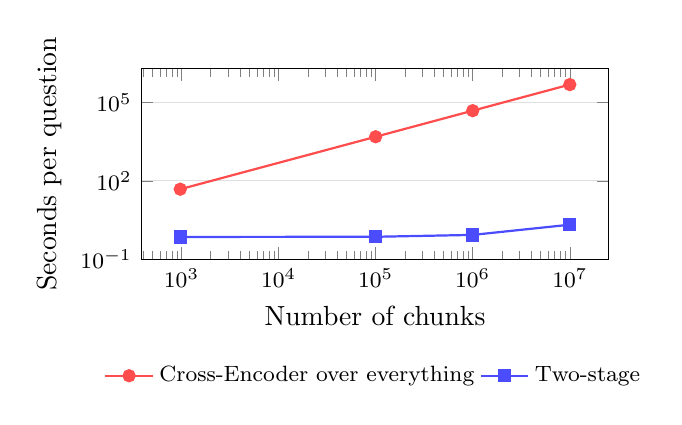
\begin{tikzpicture}
\begin{semilogyaxis}[width=0.62\linewidth,height=4cm,
  xlabel={Number of chunks},ylabel={Seconds per question},
  xmode=log,log basis x=10,ymin=0.1,ymax=2e6,
  legend style={font=\footnotesize,at={(0.5,-0.5)},anchor=north,legend columns=2,draw=none},
  ymajorgrids=true,grid style={gray!25},tick label style={font=\footnotesize}]
\addplot[red!70,thick,mark=*] coordinates {(971,48) (1e5,4924) (1e6,49244) (1e7,492444)};
\addplot[blue!70,thick,mark=square*] coordinates {(971,0.71) (1e5,0.72) (1e6,0.85) (1e7,2.09)};
\legend{Cross-Encoder over everything, Two-stage}
\end{semilogyaxis}
\end{tikzpicture}
\end{center}

The Bi-Encoder does its heavy work only once, when the index is built. After that, each question needs just one encoding and a fast search. That is why I use two stages: the Bi-Encoder quickly narrows the whole collection down to 10 chunks, and the slower Cross-Encoder only reorders those 10. The downside is that if the first stage misses the right chunk, as with Q24, Q26 and Q41, the second stage cannot bring it back.

\textbf{Limitations:} I wrote and judged all 49 questions myself on one document; I corrected the gold lists for Q40 and Q49 after reading the answers; large-scale timings are extrapolated.

\section*{Conclusion}
Re-ranking raised Hit@3 from 0.67 to 0.84 and correct answers from 6 to 14 (of 23), mostly on negation, exception and keyword-trap questions. It costs about 0.7\,s per query on CPU, sometimes demotes the most exact rule, and cannot recover chunks the first stage misses. Still, the two-stage design gives the best balance of speed and accuracy.

\end{document}
